%!TEX root = ../dissertation.tex
%
%\begin{savequote}[75mm]
%Re: The atoms in this table are in \emph{equilibrium}.
%\qauthor{-Dr. Soonwon Choi}
%\end{savequote}

\chapter{Chapter 5 Calculations}
\label{appendix:Ch5Cal}

\newpage{}

\section{Scaling and limitations of configurational correlator}


The configurational correlator $C$ studied in the text has a finite upper bound unlike the configurational entanglement entropy $S_c$. This can be seen from the inequality below:

\begin{equation}
\begin{aligned}
C &= \sum_{n=0}^N p_n \sum_{\{A_n\},\{B_n\}} \left | p(A_{n} \otimes B_{n}) + p(A_{n}) p(B_{n}) \right |\\
 &\leq\sum_{n=0}^N p_n \sum_{\{A_n\},\{B_n\}} \left | p(A_{n} \otimes B_{n})\right | + \left | p(A_{n}) p(B_{n}) \right | = 2
\end{aligned}
\end{equation}

where the last equality is enforced by the normalization of the probability distributions. This bound of $C\leq2$ can be shown to be a tight upper bound in large Hilbert space dimensions for a maximally mixed reduced density matrix, where the two probability distributions are perfectly correlated. Let us consider the maximally mixed reduced density matrix in the Schmidt basis, with $p^{(n)}_a,p^{(n)}_b = 1/N$ and $p^{(n)}_{a,b} \in \{1/N, 0\}$. For simplicity, let us consider the case where $p_n=1$ for one $n_0$ and $p_n=0$ for all other $n$. We therefore drop all superscripts of $n$. 
\begin{equation}
\begin{aligned}
C &= \sum_{\{A\},\{B\}} \left| p(A\otimes B) - p(A) p(B) \right|  \\
&\leq \sum_{a,b = 1}^N \left |\frac{1}{N} - \frac{1}{N^2} \right | + \sum_{a,b = N+1}^{N^2} \left | 0 - \frac{1}{N^2} \right | \\ 
&= N \left (\frac{1}{N} \right ) \left | 1 - \frac{1}{N} \right | +\left ( N^2 - N \right ) \frac{1}{N^2} \\
&= \frac{N-1}{N} + 1 - \frac{1}{N} = 2 \left (1-\frac{1}{N} \right)
\end{aligned}
\end{equation}

However, even with this bound, we find that the configurational entanglement entropy $S_c$ and $C$ are remarkably linear when $S_c$ is relatively small. It is also worth noting that the upper bound for the case shown above in entropy is also bounded by $\log(N)$. This temptingly suggests that in some cases a relationship could be made where perhaps $S_c \sim \log(1-C/2)$.

%\subsection{Interaction de
%\begin{figure}[ht!]
%		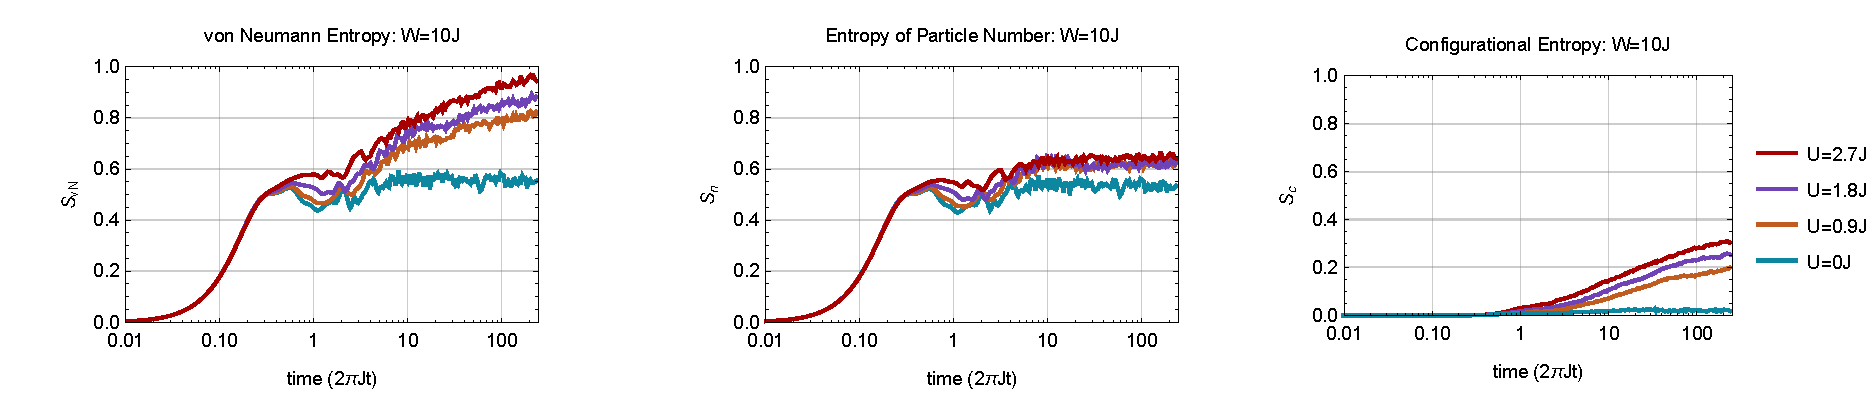
\includegraphics[width=\columnwidth]{figures/ch5/Svn_Row.pdf} 
%		\caption{\textbf{Interaction dependence a,}  }
%		\label{fig:svnRow}	
%\end{figure}

%\section{Measurements compared to l-bit picture}
%
%use other example of $\frac{1}{\mathcal{N}} \left ( \hat{\mathcal{L}}_0^\dagger+\hat{\mathcal{L}}_1^\dagger \right ) \otimes  \left ( \hat{\mathcal{L}}_2^\dagger+\hat{\mathcal{L}}_3^\dagger \right ) $
